
\section{A Pivotal Moment}
% Based on this Google Doc: 
% https://docs.google.com/document/d/1pJMU7AzuoaGf7Kegx8K9HmPANkRP2mbsWYEfkA722Cc/edit?usp=sharing


Our society currently faces the most profound and deeply disruptive public health crisis in modern history. As communities across the world grapple with the COVID-19 pandemic, scientific advances spanning biochemistry and epidemiology to manufacturing and data engineering offer hope—and a spectrum of guidance is unfolding in an effort to respond to monumental shifts in our daily lives. The rising demand for data and the emerging efforts to responsibly collect, share, and analyze information across traditional boundaries play a vital role in our next steps.  

From facilitating dialogue and decision making, to underscoring the importance of a shared, honest assessment of where we are in our collective fight against the pandemic, data are now more important than ever. Our computational capacity and the value that we as a community can generate through data science are fundamentally crucial to our resilience. As we look to transition from crisis response to longer-term recovery, we have an unprecedented opportunity to re-imagine a new data-enabled future.

\begin{figure}
    \centering
    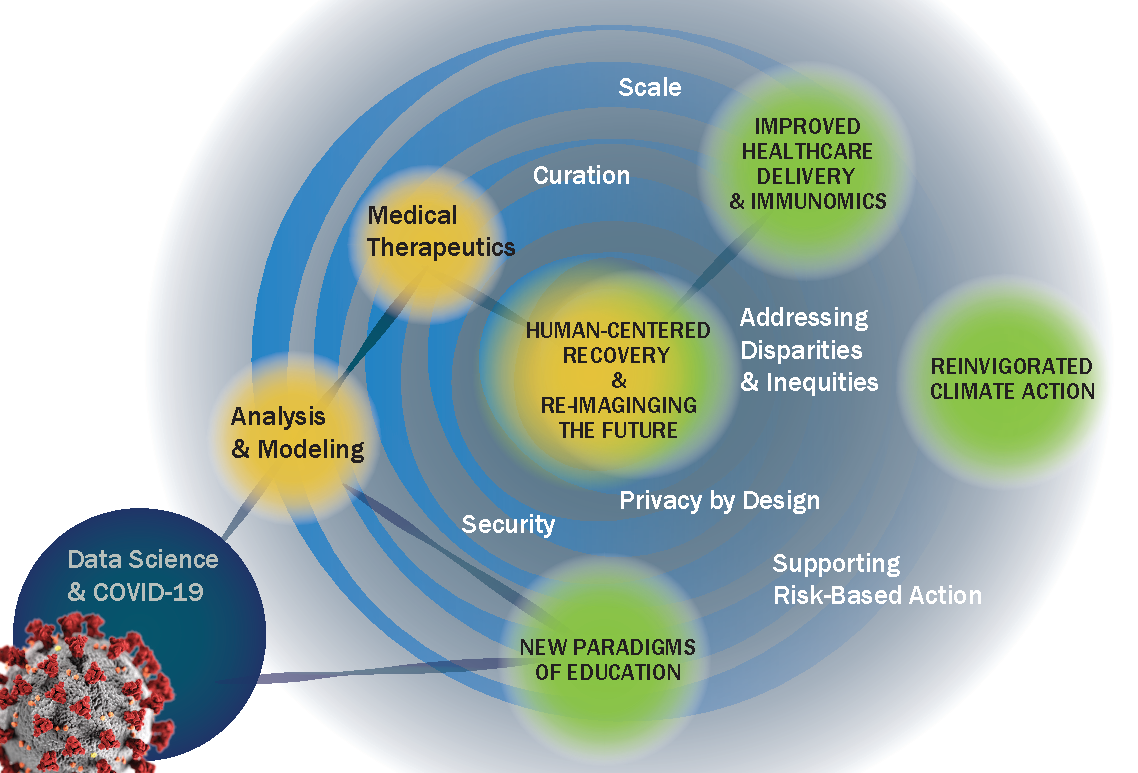
\includegraphics[width=0.75\textwidth]{figs/covid19_landscape.pdf}
    \caption{\textbf{Supporting Public Health.} The COVID-19 pandemic surfaces challenges where data science can enable new insights within a human-centered context. Current efforts, ranging from data analysis and predictive modeling to risk communication, set the stage for recovery and a new future, reinvigorated with critical questions and opportunities.}
  %  \label{fig:placesExamples}
\end{figure}
